% ---------------------------------------------------------------------------
% Case studies.
%
% The tables below are AUTO-GENERATED -- do not edit them by hand, edit the
% generating scripts (captions included) and re-run:
%
%   python Code/replication_ak91.py              -> iteration4/ak91_replication.tex
%   python Code/replication_ak91_sensitivity.py  -> iteration4/ak91_sensitivity.tex
%                                                   images/graphs/ak91_seed_sensitivity.png
%   python Code/replication_ae98.py              -> iteration4/ae98_replication.tex
%   python Code/replication_ae98_sensitivity.py  -> iteration4/ae98_sensitivity.tex
%                                                   images/graphs/ae98_seed_sensitivity_*.png
%
% Data provenance is documented in data/AngristKreuger1991/readme.txt and
% data/AngristEvans1998/README.md.
% ---------------------------------------------------------------------------

\section{Case Studies}
\label{sec:case_studies}

The simulations of Section~\ref{ss:simulation_results} evaluated the estimators and tests on data generated to satisfy \ref{ass:exog}--\ref{ass:moments} by construction, with the instrument strength conditions holding or failing by design. This section applies the same procedures to two instrumental variable studies, where neither the tail behaviour nor the instrument strength is under our control.

The two applications are chosen to complement each other regarding instrument strength. \citet{angrist1991does} instrument years of schooling with quarter of birth. There $\mu_{ZX}$ is small relative to $\sigma_{ZX}$ and every finite-sample strength condition of Sections~\ref{sec:standard_iv}--\ref{sec:mor} fails. \citet{angrist1998children} instrument family size with the sex composition of the first two children. There instrument is stronger relative to the noise and all three strength conditions hold. Reading the two studies together therefore separates what the estimators do when the theory applies from what they do when it does not.

The purpose of this exercise is not to check whether the MoM-based estimators recover the published numbers, but rather to check what these methods buy, and cost, on real data.

\subsection{Empirical Strategy}
\label{ss:case_strategy}

\subsubsection{Mapping the applications into the scalar model}

The theory developed concerns $Y_i = \beta X_i + \varepsilon_i$ with a single instrument $Z_i$ and $\beta = \mu_{ZY}/\mu_{ZX}$. Both applications are therefore taken in their Wald form, that is, the just-identified specification with a single binary instrument and no covariates. In each case the published paper reports this specification alongside its covariate-adjusted counterparts, which makes the replication target unambiguous: Panel~B of Table~III in \citet{angrist1991does} and columns~(1)--(2) of Table~5 in \citet{angrist1998children}.

Both papers write their models with an intercept. Our methods have been developed without an intercept, so we demean the three variables at the full-sample level before applying any procedure,
\[
    Y_i \leftarrow Y_i - \bar{Y}, \qquad
    X_i \leftarrow X_i - \bar{X}, \qquad
    Z_i \leftarrow Z_i - \bar{Z}.
\]
With a binary instrument the sample ratio $\hat{\mu}_{ZY}/\hat{\mu}_{ZX}$ of the demeaned variables is then algebraically identical to the Wald estimator $(\bar{Y}_1 - \bar{Y}_0)/(\bar{X}_1 - \bar{X}_0)$, so the Mean IV estimator of Section~\ref{sec:standard_iv} reproduces the published point estimate. Demeaning also keeps the moment $W_i(\beta_0) = Z_i(Y_i - \beta_0 X_i)$ of Section~\ref{ss:inversion} centred at zero under $H_0$, which would not hold if the intercept were left in.

The interpretation of the MoM-based estimators are the same as the Wald estimators; the estimands capture the local average treatment effect since they estimate the same ratio of population moments.

\subsubsection{Blocking, and why the partition is randomised}
\label{sss:partition}

\subsubsection{Reported quantities}

For each application we report, at $\delta = 0.05$ throughout: the replication of the published table; the four point estimators (Mean~IV, Ratio-of-Medians, Median-of-Ratios, and the Catoni competitor of Section~\ref{sec:sim_catoni}); the three feasible confidence sets (MoM-AR with the robust scale estimate, the self-normalised AR test, and the standard AR test as a baseline); and a plug-in check of the finite-sample strength conditions. The oracle MoM-AR test of Theorem~\ref{thm:mom_ar_size} is not feasible on real data, since $\sigma_{Z\varepsilon}$ is unknown, so only its feasible counterpart as developed earlier appears here.


\subsection{The Causal Effect of Compulsory School Attendance on Earnings}
\label{ss:ak91}

\subsubsection{Data and replication}

\citet{angrist1991does} exploit the fact that compulsory schooling laws are measured with regards to age, and not grade completed. Therefore, children born earlier in the calendar year reach the legal dropout age having completed less schooling, so quarter of birth shifts educational attainment without, the authors argue, affecting earnings through any other channel. We replicate Panel~B of their Table~III, the 1980 Census sample of men born 1930--1939, with $Y$ the log weekly wage, $X$ years of education and $Z$ an indicator for birth in the first quarter.

Table~\ref{tab:ak91_panelB} reproduces the published group means, differences and Wald estimate. The posted extract contains $329{,}509$ observations against the $327{,}509$ reported in the paper, as it is the sample used for their Table~V; every reported quantity nonetheless matches to the precision printed in the original.

\todo[inline]{Why is there a 2000 observation discrepancy?}


% Auto-generated by Code/replication_ak91.py -- do not edit by hand.
% Replication of Angrist & Krueger (1991), Table III, Panel B.

\begin{table}[htbp]
\centering
\caption{Replication of \citet{angrist1991does}, Table~III, Panel~B (1980 Census, men born 1930--1939). The posted extract has $n = 329{,}509$ observations against the published 327{,}509; standard errors in parentheses.}
\label{tab:ak91_panelB}
\begin{tabular}{lcccc}
\toprule
 & \multicolumn{2}{c}{Replicated} & \multicolumn{2}{c}{Published} \\
\cmidrule(lr){2-3}\cmidrule(lr){4-5}
 & Estimate & (s.e.) & Estimate & (s.e.) \\
\midrule
$\ln$(wkly.\ wage), born Q1 & 5.8916 &  & 5.8916 &  \\
$\ln$(wkly.\ wage), born Q2--4 & 5.9027 &  & 5.9027 &  \\
\quad difference & -0.01110 & (0.00274) & -0.01110 & (0.00274) \\
Education, born Q1 & 12.6881 &  & 12.6881 &  \\
Education, born Q2--4 & 12.7969 &  & 12.7969 &  \\
\quad difference & -0.1088 & (0.0133) & -0.1088 & (0.0132) \\
Wald return to education & 0.1020 & (0.0240) & 0.1020 & (0.0239) \\
OLS return to education & 0.0709 & (0.00034) & 0.0709 & (0.0003) \\
\bottomrule
\end{tabular}
\end{table}

\begin{table}[htbp]
\centering
\caption{Robust IV estimates and 95\% confidence sets for the return to education, AK91 extract ($\delta = 0.05$; demeaned $Y$, $X$, $Z$; $k = 24$, $m = 13{,}729$). The MoM-AR test uses the feasible robust scale estimate $\hat\sigma_{Z\varepsilon} = 0.3429$; the oracle version is infeasible on real data.}
\label{tab:ak91_robust}
\begin{tabular}{lc}
\toprule
Estimator & $\hat\beta$ \\
\midrule
Wald / Mean IV & 0.1020 (0.0240) \\
Ratio-of-Medians ($k=30$) & 0.1023 \\
Median-of-Ratios ($k=24$) & 0.0584 \\
Catoni ratio ($\delta/2$ per coordinate) & 0.1018 \\
\midrule
Test & 95\% confidence set \\
\midrule
MoM-AR (feasible) & $[-0.1923,\, 0.3839]$ \\
SN-AR & $[-0.0097,\, 0.1744] \cup [0.1761,\, 0.1935] \cup [0.2221,\, 0.2325]$ \\
AR (standard) & $[0.0554,\, 0.1525]$ \\
\bottomrule
\end{tabular}
\end{table}


\subsubsection{Instrument strength}
\label{sss:ak91_strength}

The plug-in moments of the demeaned data are $\hat{\mu}_{ZX} = -0.0203$ and $\hat{\sigma}_{ZX}^2 = 2.031$, so $\hat{\sigma}_{ZX}^2/\hat{\mu}_{ZX}^2 \approx 4{,}900$. Every finite-sample condition of the point estimators fails.The standard IV condition~\eqref{eq:iv_strength} requires $n \geq 789{,}667$ against the $329{,}509$ available; the Median-of-Ratios condition~\eqref{eq:mor_strength} requires a block size $m \geq 157{,}933$ against $m = 13{,}729$; and the Ratio-of-Medians condition~\eqref{eq:rom_strength} requires $m > 19{,}742$ against $m = 10{,}983$.

\subsubsection{Robust estimates and confidence sets}
\todo[inline]{mention seed chosen is ``1971"}


Table~\ref{tab:ak91_robust} reports the four estimators and the three confidence sets for one documented partition.

The Catoni and Ratio-of-Medians estimators both agree closely with the Wald estimator, while the Median-of-Ratios sits below them at this seed. The feasible MoM-AR set is far wider than the standard AR set and includes. The self-normalised AR test is a union of three intervals, one of which also includes zero. Additionally, none of the confidence sets reject the Wald value.

The consequence is clear; the point estimate of \citet{angrist1991does} is reproduced exactly, and nothing here contradicts their conclusion. The finite-sample robust tests are simply uninformative in this application. Their confidence sets are wide enough to contain both zero and the Wald estimate, which is the price.


\subsubsection{Partition sensitivity}
\label{sss:ak91_sensitivity}

Table~\ref{tab:ak91_sensitivity} and Figure~\ref{fig:ak91_sensitivity} summarise $B = 1{,}000$ independent partitions of the same data.

The dispersion induced by the partition is of the same order as the sampling uncertainty of the Wald estimator: the Median-of-Ratios estimate has a standard deviation of $0.019$ across partitions and ranges over $[0.028, 0.150]$, against a Wald standard error of $0.024$. As stated earlier, Catoni's estimator is essentially partition free. The block means $\hat{\mu}_{ZX}^{(j)}$ share a sign in only $30.4\%$ of partitions, so the sufficient condition of Proposition~\ref{prop:mono_det} usually fails, and the self-normalised confidence set is a union of several intervals in $14.6\%$ of draws. The feasible MoM-AR set excludes zero in $1.8\%$ of partitions against $91.6\%$ for the self-normalised set and $100\%$ for the partition-free standard AR test.

\todo[inline]{Discuss consequence of how sensitive inference is on seed}

% Auto-generated by Code/replication_ak91_sensitivity.py -- do not edit by hand.

\begin{table}[htbp]
\centering
\small
\setlength{\tabcolsep}{4pt}
\caption{Partition sensitivity on the AK91 extract: $B = 1{,}000$ independent random partitions, each shared by all MoM-based procedures ($\delta = 0.05$). The partition-free Wald estimate is $0.1020$. Top panel: dispersion of the point estimates across partitions. Bottom panel: rejection and shape frequencies of the 95\% confidence sets; the standard AR test does not depend on the partition and is shown for reference.}
\label{tab:ak91_sensitivity}
\begin{tabular}{lccccc}
\toprule
Estimator & Median & SD & Q$_{0.05}$ & Q$_{0.95}$ & Range \\
\midrule
Median-of-Ratios & 0.0992 & 0.0189 & 0.0666 & 0.1284 & [0.0280, 0.1496] \\
Ratio-of-Medians & 0.1013 & 0.0211 & 0.0686 & 0.1373 & [0.0409, 0.2036] \\
Catoni ratio & 0.1018 & 0.0000 & 0.1018 & 0.1019 & [0.1018, 0.1019] \\
\midrule
Test & \multicolumn{1}{c}{\% rej.\ $0$} & \multicolumn{1}{c}{\% rej.\ $\beta_{\mathrm{OLS}}$} & \multicolumn{1}{c}{\% split} & \multicolumn{1}{c}{\% unb.} & \multicolumn{1}{c}{Med.\ len.} \\
\midrule
MoM-AR (feasible) & 1.8 & 0.0 & 0.1 & 0.0 & 0.431 \\
SN-AR & 91.6 & 10.1 & 14.6 & 0.0 & 0.145 \\
AR (standard) & 100.0 & 0.0 & 0.0 & 0.0 & 0.097 \\
\bottomrule
\end{tabular}
\end{table}


\begin{figure}[htbp]
  \centering
  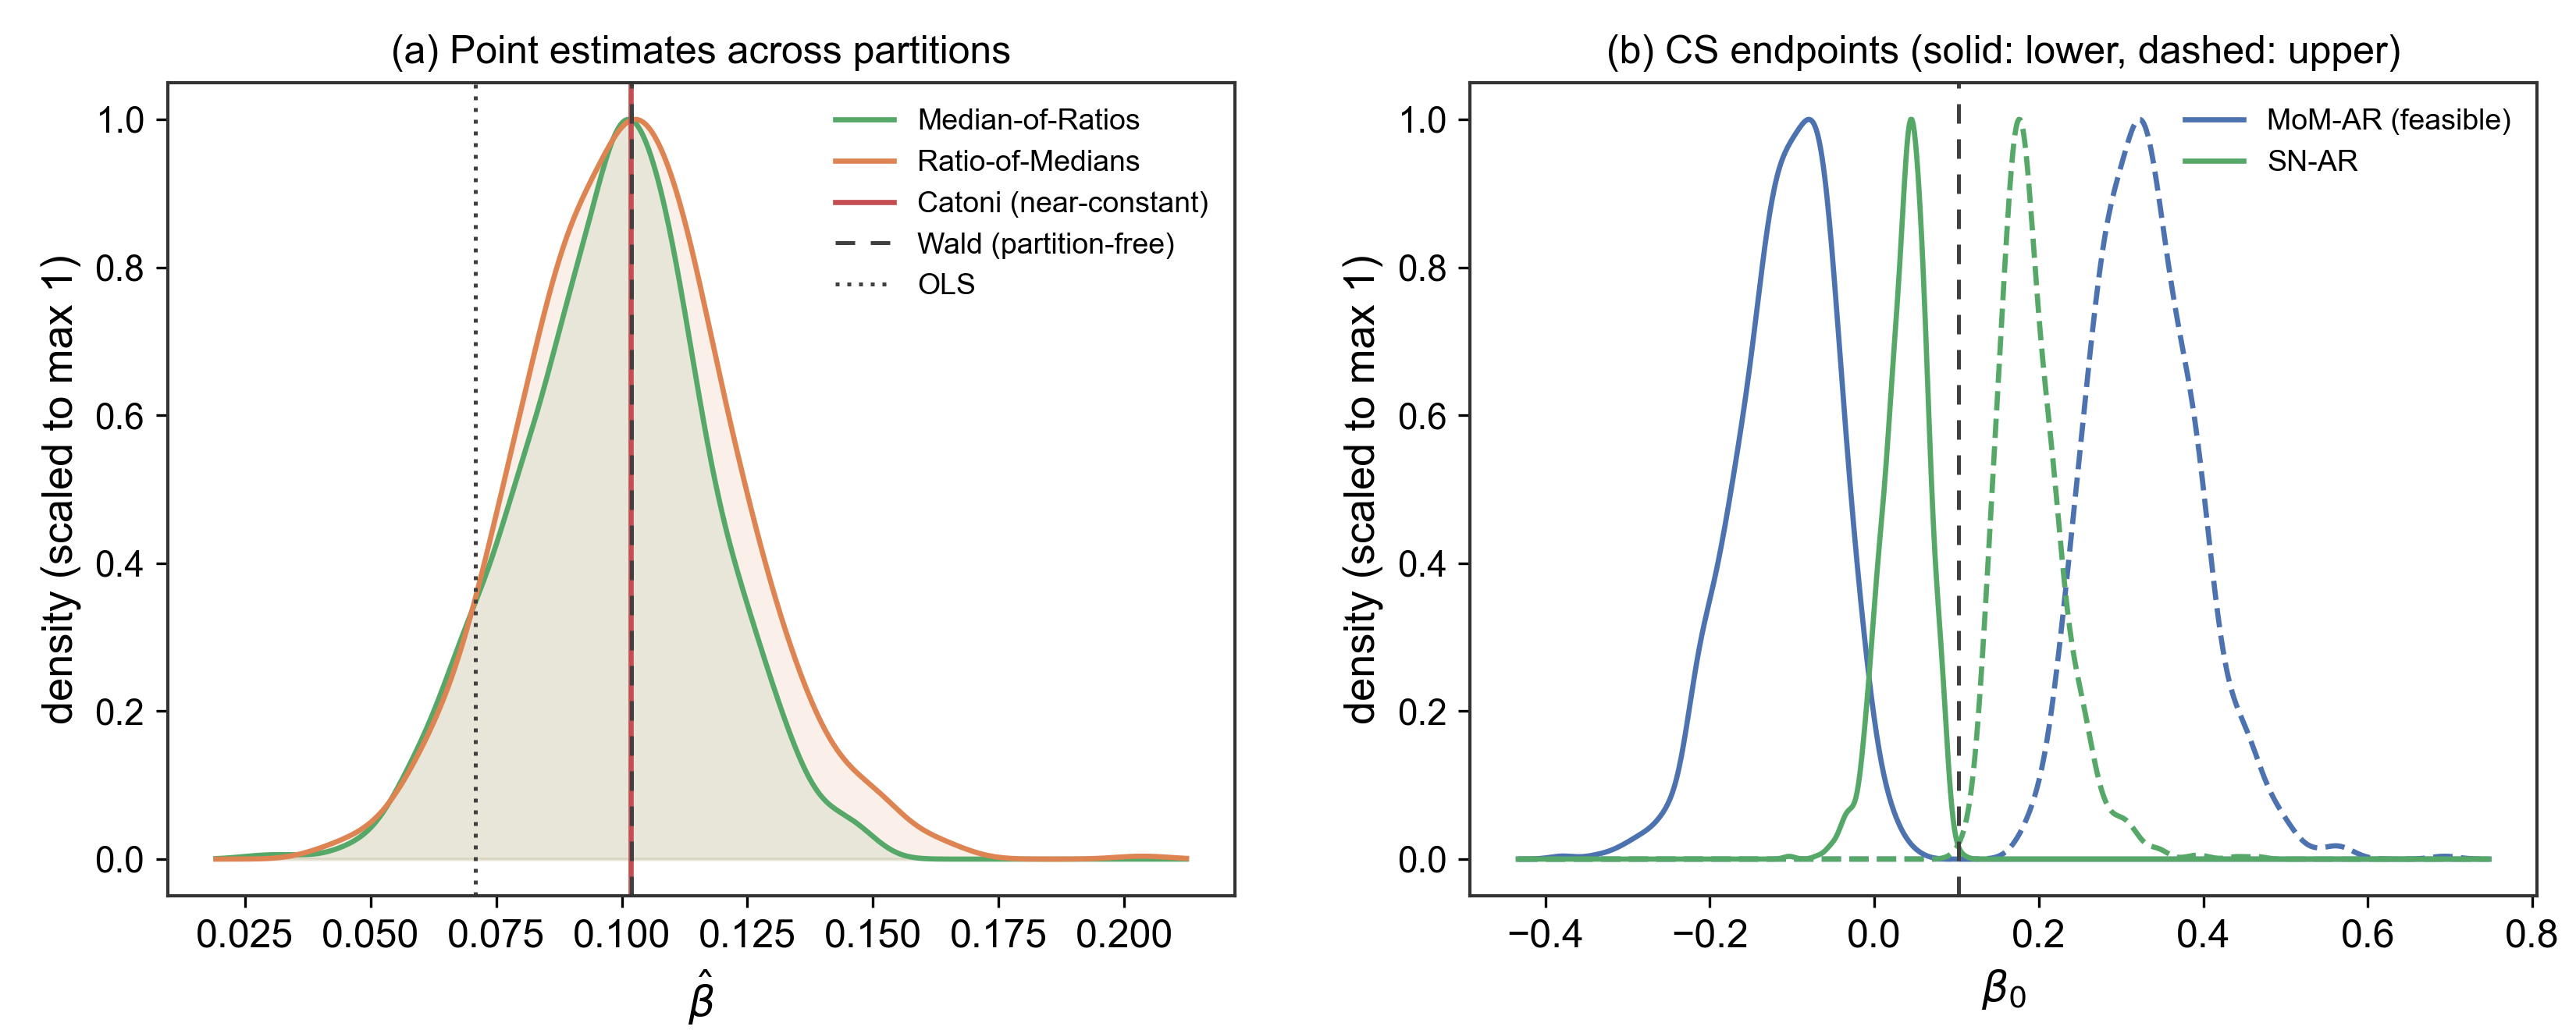
\includegraphics[width=\textwidth]{images/graphs/ak91_seed_sensitivity.png}
  \caption{Partition sensitivity on the \citet{angrist1991does} extract over $B = 1{,}000$ random partitions. Panel~(a): kernel density estimates of the point estimates, each scaled to unit maximum, with the partition-free Wald and OLS values marked. Panel~(b): densities of the outer endpoints of the 95\% confidence sets (solid: lower, dashed: upper).}
  \label{fig:ak91_sensitivity}
\end{figure}

\subsubsection{Aggregated estimates and confidence sets}
\label{sss:ak91_aggregated}

Table~\ref{tab:ak91_aggregated} applies the aggregation of Section~\ref{sec:aggregation} to the $B = 1{,}000$ partitions of the previous subsection, reporting the aggregated estimator of Definition~\ref{def:randomised} and the aggregated confidence set of Corollary~\ref{cor:agg_cs}. Every permutation drawn enters the same aggregate, so the table has no seed left to report, and it is directly comparable with Table~\ref{tab:ak91_robust}, which is the same quantities on one partition.

\todo[inline]{Expand: Aggregation buys back most of what Section~\ref{sss:ak91_sensitivity} showed the seed was costing. The Median-of-Ratios estimate moves from $0.0584$ on the documented partition, one draw from a range of $[0.028, 0.150]$, to $0.0992$, within $0.003$ of the partition-free Wald value $0.1020$; Ratio-of-Medians lands at $0.1013$. The self-normalised set is the sharper illustration: on one partition it was a union of three intervals, and whether it excluded zero was a function of the seed in $8.4\%$ of draws. Aggregated it is the single interval $[0.0413, 0.1829]$, it excludes zero, and there is no seed left to vary. Nothing is paid in width for that: the aggregated sets have essentially the median length of the per-partition sets, $0.142$ against a median of $0.15$ for the self-normalised test and $0.428$ against $0.43$ for MoM-AR. What aggregation does not repair is the conservativeness of $\tau_n(\delta)$, so the feasible MoM-AR set still contains both zero and the Wald estimate, exactly as in Table~\ref{tab:ak91_robust}. Note also that the aggregated set is guaranteed at $2\delta$ rather than $\delta$, so a like-for-like comparison would run the underlying test at $\delta/2$ (Remark~\ref{rem:agg_price}).}

% Auto-generated by Code/replication_ak91_sensitivity.py -- do not edit by hand.

\begin{table}[htbp]
\centering
\caption{Aggregated estimates and the aggregated 95\% confidence set on the AK91 extract, over all $B = 1{,}000$ random partitions of Table~\ref{tab:ak91_sensitivity} (Definition~\ref{def:randomised} and Corollary~\ref{cor:agg_cs}, $\delta = 0.05$; $k = 24$ for MoR and the tests, $k = 30$ for RoM). Table~\ref{tab:ak91_robust} is the same quantities on a single partition. The Wald estimator and the standard AR test do not depend on the partition and are shown for reference; by Corollary~\ref{cor:agg_cs} the aggregated set is guaranteed at $2\delta$, not $\delta$.}
\label{tab:ak91_aggregated}
\begin{tabular}{lc}
\toprule
Aggregated estimator & $\widetilde{\beta}_B$ \\
\midrule
Median-of-Ratios & 0.0992 \\
Ratio-of-Medians & 0.1013 \\
Wald / Mean IV (partition-free) & 0.1020 \\
\midrule
Aggregated test & 95\% confidence set \\
\midrule
MoM-AR (feasible) & $[-0.1031,\, 0.3245]$ \\
SN-AR & $[0.0413,\, 0.1829]$ \\
AR (standard, partition-free) & $[0.0554,\, 0.1525]$ \\
\bottomrule
\end{tabular}
\end{table}


\subsection{The Causal Effect of Family Size on Parental Labour Supply}
\label{ss:ae98}

\subsubsection{Data and replication}

\citet{angrist1998children} estimate the effect of childbearing on parents' labour supply, instrumenting an indicator for having more than two children with an indicator for the first two children having the same sex. Parents with two same-sex children are more likely to have a third, while the sex mix itself is as good as randomly assigned, which is the identifying claim. We replicate columns~(1)--(2) of their Table~5, which is the 1980 Census sample of all women aged 21--35 with two or more children, for the five labour-supply outcomes.

Table~\ref{tab:ae98_table5} reports the replication. The reconstructed sample contains $394{,}840$ observations against the $394{,}835$ of the published table, a five-observation discrepancy of the posted archive also reported by \citet{farbmacher2018twin}, whose selection rules we follow. The first stage is $0.0595$ against a published $0.0600$, and all five Wald estimates match at printed precision.

% Auto-generated by Code/replication_ae98.py -- do not edit by hand.
% Replication of Angrist & Evans (1998), Table 5, 1980 PUMS, all women.

\begin{table}[htbp]
\centering
\caption{Replication of \citet{angrist1998children}, Table~5, columns (1)--(2): 1980 PUMS, all women aged 21--35 with two or more children, \emph{Same sex} instrument, \emph{More than 2 children} as endogenous regressor. Reconstructed sample $n = 394{,}840$ against the published 394{,}835 (five-observation archive discrepancy documented by \citet{farbmacher2018twin}). Standard errors in parentheses; Wald SEs by the delta method.}
\label{tab:ae98_table5}
\begin{tabular}{lcccc}
\toprule
 & \multicolumn{2}{c}{Replicated} & \multicolumn{2}{c}{Published} \\
\cmidrule(lr){2-3}\cmidrule(lr){4-5}
 & Estimate & (s.e.) & Estimate & (s.e.) \\
\midrule
\emph{More than 2 children} & 0.0595 & (0.0016) & 0.0600 & (0.0016) \\
\emph{Number of children} & 0.0754 & (0.0026) & 0.0765 & (0.0026) \\
\midrule
Worked for pay, difference & -0.0079 & (0.0016) & -0.008 & (0.0016) \\
\quad Wald & -0.132 & (0.026) & -0.133 & (0.026) \\
Weeks worked, difference & -0.3787 & (0.0709) & -0.3826 & (0.0709) \\
\quad Wald & -6.360 & (1.181) & -6.38 & (1.17) \\
Hours/week, difference & -0.3089 & (0.0602) & -0.311 & (0.0602) \\
\quad Wald & -5.187 & (1.006) & -5.18 & (1.0) \\
Labor income, difference & -130.3 & (34.4) & -132.5 & (34.4) \\
\quad Wald & -2188.3 & (573.6) & -2208.8 & (569.2) \\
ln(Family income), difference & -0.0016 & (0.0041) & -0.0018 & (0.0041) \\
\quad Wald & -0.026 & (0.069) & -0.029 & (0.068) \\
\bottomrule
\end{tabular}
\end{table}

\begin{table}[htbp]
\centering
\caption{Robust IV estimates and 95\% confidence sets, AE98 1980 all-women sample ($\delta = 0.05$; demeaned $Y$, $X$, $Z$; one shared random partition, $k = 24$, $m = 16{,}451$ for MoR and the tests, $k = 30$ for RoM). The MoM-AR test uses the feasible robust scale estimate; the oracle version is infeasible on real data.}
\label{tab:ae98_robust}
\begin{tabular}{lcccc}
\toprule
Outcome & Wald/Mean IV & MoR & RoM & Catoni \\
\midrule
Worked for pay & -0.1318 & -0.1118 & -0.1398 & -0.1318 \\
Weeks worked & -6.3596 & -6.2532 & -7.7001 & -6.3595 \\
Hours/week & -5.1872 & -4.8504 & -6.6122 & -5.1871 \\
Labor income & -2188.3 & -1734.1 & -2860.9 & -2188.4 \\
ln(Family income) & -0.0262 & -0.0436 & 0.0481 & -0.0262 \\
\midrule
Outcome & \multicolumn{2}{c}{MoM-AR (feasible)} & SN-AR & AR (standard) \\
\midrule
Worked for pay & \multicolumn{2}{c}{$[-0.307,\, 0.072]$} & $[-0.170,\, -0.051]$ & $[-0.184,\, -0.080]$ \\
Weeks worked & \multicolumn{2}{c}{$[-18.46,\, 5.48]$} & $[-10.32,\, -2.47]$ & $[-8.68,\, -4.04]$ \\
Hours/week & \multicolumn{2}{c}{$[-14.88,\, 3.77]$} & $[-8.72,\, -2.49]$ & $[-7.16,\, -3.22]$ \\
Labor income & \multicolumn{2}{c}{$[-5013,\, 1281]$} & $[-2764,\, -683]$ & $[-3313,\, -1061]$ \\
ln(Family income) & \multicolumn{2}{c}{$[-1.104,\, 1.194]$} & $[-0.362,\, 0.262]$ & $[-0.161,\, 0.109]$ \\
\bottomrule
\end{tabular}
\end{table}


\subsubsection{Instrument strength}

Here $\hat{\mu}_{ZX} = 0.0149$ and $\hat{\sigma}_{ZX}^2 = 0.0598$, so $\hat{\sigma}_{ZX}^2/\hat{\mu}_{ZX}^2 \approx 270$, roughly eighteen times smaller than in Section~\ref{sss:ak91_strength}. The standard IV condition~\eqref{eq:iv_strength} requires $n \geq 43{,}219$ and is met with $394{,}840$ observations; the Median-of-Ratios condition~\eqref{eq:mor_strength} requires $m \geq 8{,}644$ and is met with $m = 16{,}451$; the Ratio-of-Medians condition~\eqref{eq:rom_strength} requires $m > 1{,}080$ and is met with $m = 13{,}161$.


\subsubsection{Robust estimates and confidence sets}

Table~\ref{tab:ae98_robust} reports the four estimators and the three confidence sets for one documented partition. The estimators agree closely for the bounded outcomes and less closely for the unbounded ones. For Labour income the Median-of-Ratios estimate is $21\%$ below the Wald estimate and the Ratio-of-Medians estimate $31\%$ above it, and for ln(Family income) the latter reverses sign. The ordering follows the tail behaviour of Section~\ref{sss:case_tails}, but each gap lies within roughly two partition standard deviations of Table~\ref{tab:ae98_sensitivity}, so it reflects the draw of the partition rather than the estimator.

None of the five feasible MoM-AR sets excludes zero, and all are three to five times longer than the standard AR sets. This is not a symptom of a weak instrument, since all three strength conditions hold here; at $\delta = 0.05$ the threshold $\tau_n(\delta)$ of~\eqref{eq:tau} exceeds the classical critical value by a factor $\sqrt{32\ln(1/\delta)}/1.96 \approx 5$, which accounts for essentially all of the gap. The binding constraint is the conservativeness of the threshold, not instrument strength. The self-normalised sets exclude zero for all four labour-supply outcomes and are each a single interval, in contrast with Section~\ref{ss:ak91}, where the same test returned a union of three; for ln(Family income) no procedure excludes zero, matching the null result of \citet{angrist1998children}.


\subsubsection{Partition sensitivity}
\label{sss:ae98_sensitivity}

Table~\ref{tab:ae98_sensitivity} and Figures~\ref{fig:ae98_sensitivity_workedm} and~\ref{fig:ae98_sensitivity_incomem} summarise $B = 1{,}000$ partitions of the same data. For every outcome the estimator distributions are centered on the partition-free Wald value, and the partition standard deviation is between $68\%$ and $71\%$ of the sampling standard error, $0.018$ against $0.026$ for Worked for pay. No confidence set, for any outcome or any partition, is split or unbounded. The self-normalised test excludes zero in $99\%$ or more of partitions for the three labour-supply outcomes and in $90.4\%$ for Labour income, the difference being visible in panel~(b), where the density of the upper endpoint sits clear of zero in the first case and straddles it in the second.

The contrast with Section~\ref{sss:ak91_sensitivity} is not one of magnitude, since the dispersion there is a comparable fraction of the sampling standard error. In \citet{angrist1991does} the partition determines the shape of the confidence set and moves the Median-of-Ratios estimate over $[0.028, 0.150]$, so the reported answer depends on a seed. Here, every partition delivers the same verdict for every outcome.

% Auto-generated by Code/replication_ae98_sensitivity.py -- do not edit by hand.

\begin{table}[htbp]
\centering
\caption{Partition sensitivity on the AE98 1980 all-women sample: $B = 1{,}000$ random partitions shared by all MoM-based procedures and reused across outcomes ($\delta = 0.05$). For each outcome, the top rows give the dispersion of the partition-dependent point estimates (the partition-free Wald estimate in the label); the bottom rows give rejection and shape frequencies of the 95\% confidence sets. The standard AR test is partition-free and shown for reference.}
\label{tab:ae98_sensitivity}
\small
\begin{tabular}{llccccc}
\toprule
Outcome & Estimator & Mean & SD & Q$_{0.05}$ & Q$_{0.95}$ & \\
\midrule
Worked for pay (Wald -0.1318) & Median-of-Ratios & -0.1331 & 0.0184 & -0.1641 & -0.1028 & \\
 & Ratio-of-Medians & -0.1325 & 0.0189 & -0.1638 & -0.1016 & \\
 & Catoni ratio & -0.1318 & 0.0000 & -0.1318 & -0.1318 & \\
Weeks worked (Wald -6.3596) & Median-of-Ratios & -6.4039 & 0.8206 & -7.7276 & -5.0832 & \\
 & Ratio-of-Medians & -6.3876 & 0.8753 & -7.8407 & -4.9402 & \\
 & Catoni ratio & -6.3595 & 0.0000 & -6.3595 & -6.3595 & \\
Hours/week (Wald -5.1872) & Median-of-Ratios & -5.1964 & 0.6893 & -6.3345 & -4.0640 & \\
 & Ratio-of-Medians & -5.2486 & 0.7021 & -6.4069 & -4.0759 & \\
 & Catoni ratio & -5.1871 & 0.0000 & -5.1871 & -5.1871 & \\
Labor income (Wald -2188.3) & Median-of-Ratios & -2195.0 & 395.1 & -2833.3 & -1546.7 & \\
 & Ratio-of-Medians & -2170.3 & 398.9 & -2823.9 & -1526.5 & \\
 & Catoni ratio & -2188.4 & 0.0 & -2188.4 & -2188.4 & \\
ln(Family income) (Wald -0.0262) & Median-of-Ratios & -0.0257 & 0.0469 & -0.1032 & 0.0497 & \\
 & Ratio-of-Medians & -0.0249 & 0.0487 & -0.1032 & 0.0559 & \\
 & Catoni ratio & -0.0262 & 0.0000 & -0.0262 & -0.0262 & \\
\midrule
Outcome & Test & \% rej.\ $\beta_0{=}0$ & \% rej.\ $\beta_0{=}\beta_{\mathrm{OLS}}$ & \% split & \% unb. & Med.\ len. \\
\midrule
Worked for pay & MoM-AR (feasible) & 3.5 & 0.0 & 0.0 & 0.0 & 0.469 \\
 & SN-AR & 99.3 & 1.2 & 0.0 & 0.0 & 0.144 \\
 & AR (standard, partition-free) & 100.0 & 0.0 & 0.0 & 0.0 & 0.103 \\
Weeks worked & MoM-AR (feasible) & 7.5 & 0.0 & 0.0 & 0.0 & 20.976 \\
 & SN-AR & 99.6 & 1.4 & 0.0 & 0.0 & 6.366 \\
 & AR (standard, partition-free) & 100.0 & 0.0 & 0.0 & 0.0 & 4.636 \\
Hours/week & MoM-AR (feasible) & 6.0 & 0.0 & 0.0 & 0.0 & 17.710 \\
 & SN-AR & 99.0 & 5.9 & 0.0 & 0.0 & 5.530 \\
 & AR (standard, partition-free) & 100.0 & 0.0 & 0.0 & 0.0 & 3.948 \\
Labor income & MoM-AR (feasible) & 1.1 & 0.0 & 0.0 & 0.0 & 10077 \\
 & SN-AR & 90.4 & 1.2 & 0.0 & 0.0 & 3115 \\
 & AR (standard, partition-free) & 100.0 & 0.0 & 0.0 & 0.0 & 2251 \\
ln(Family income) & MoM-AR (feasible) & 0.0 & 0.0 & 0.0 & 0.0 & 1.233 \\
 & SN-AR & 1.2 & 18.2 & 0.0 & 0.0 & 0.383 \\
 & AR (standard, partition-free) & 0.0 & 100.0 & 0.0 & 0.0 & 0.270 \\
\bottomrule
\end{tabular}
\end{table}


\begin{figure}[htbp]
  \centering
  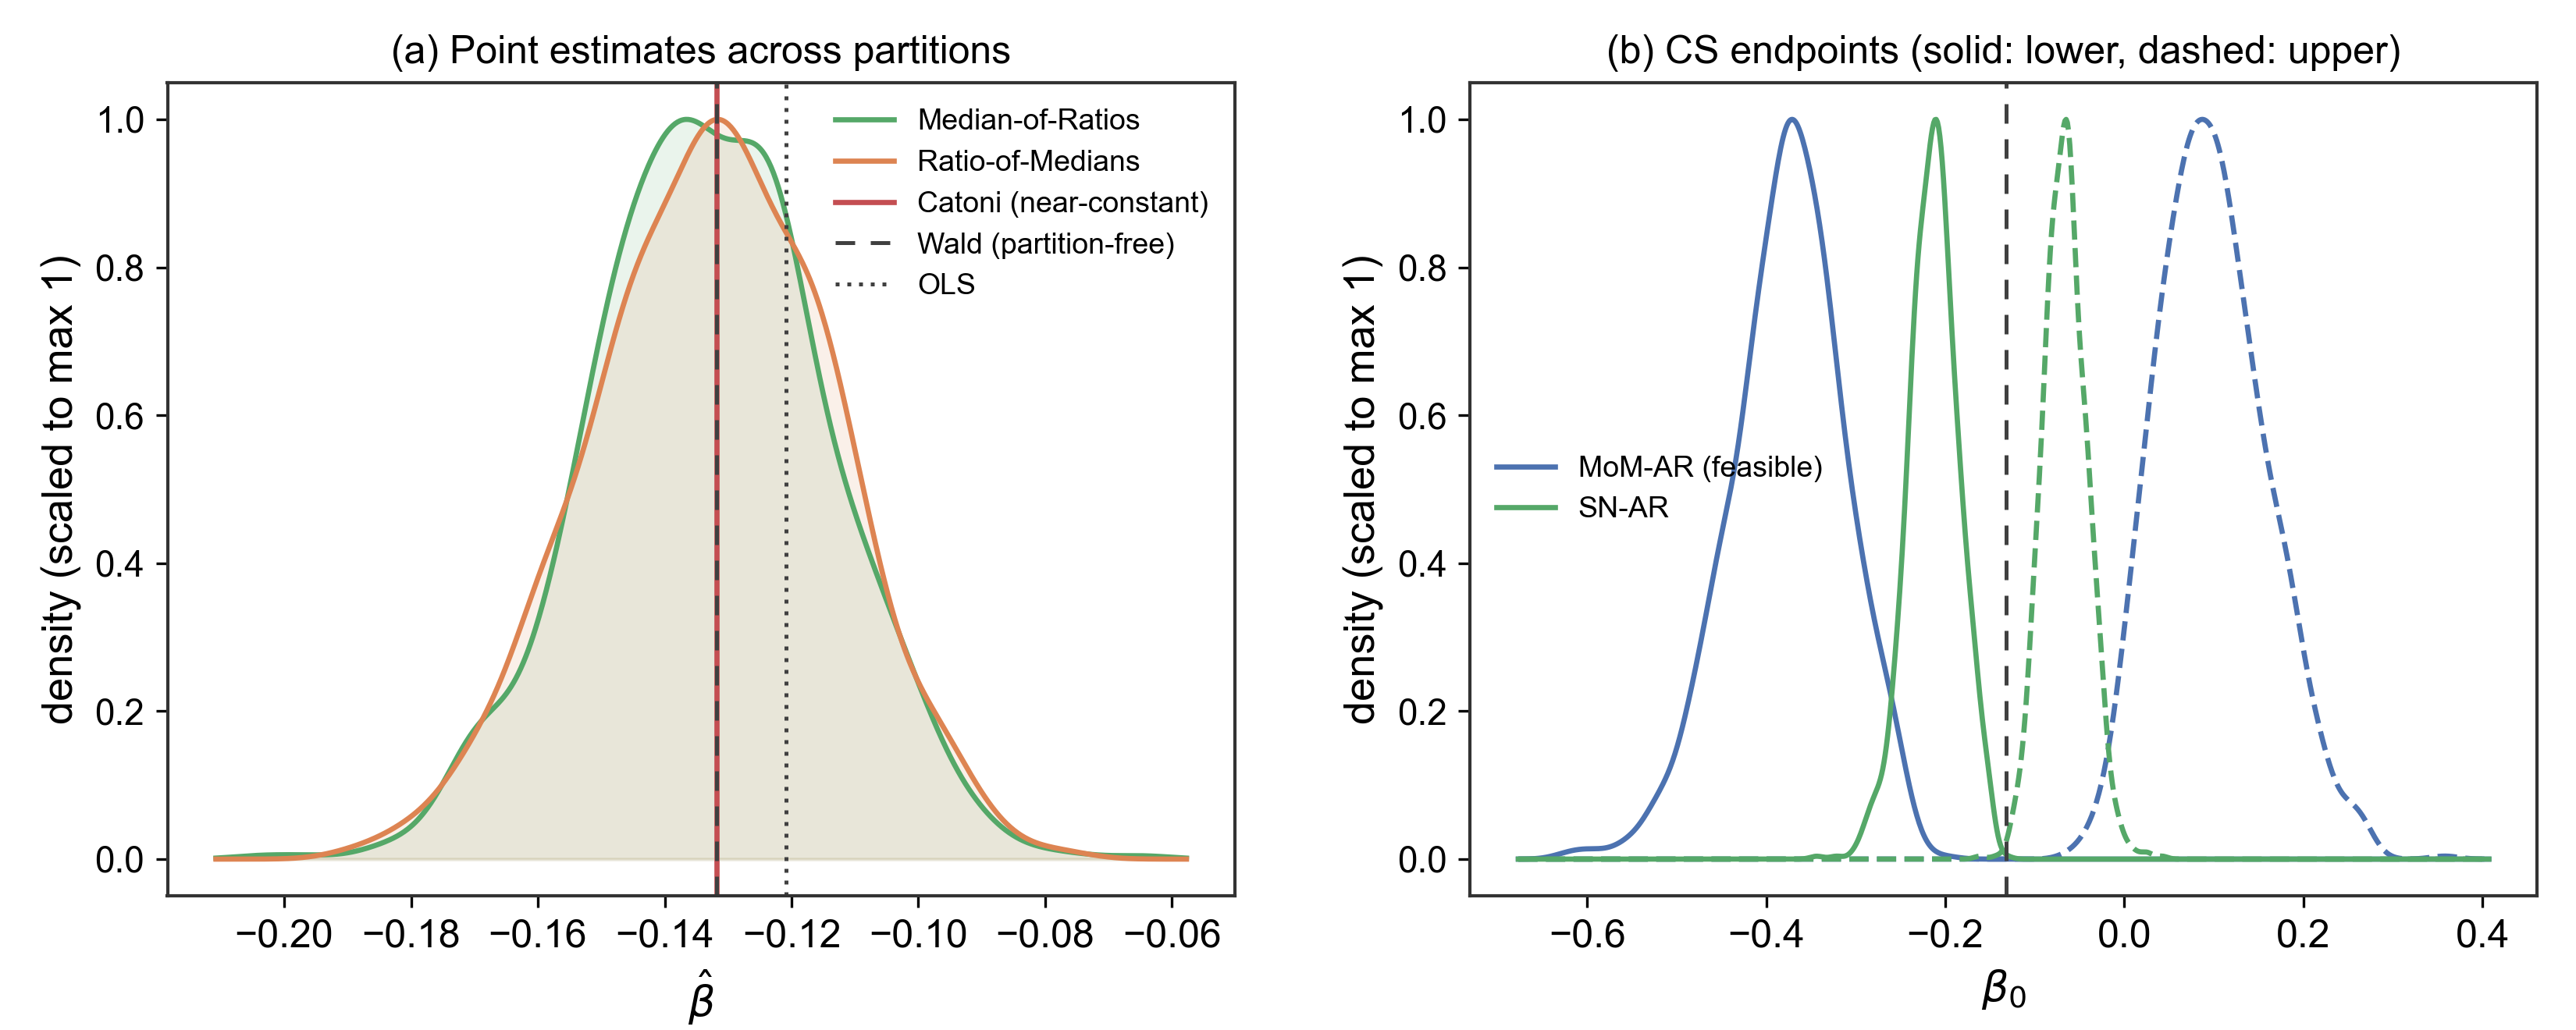
\includegraphics[width=\textwidth]{images/graphs/ae98_seed_sensitivity_workedm.png}
  \caption{Partition sensitivity for Worked for pay, \citet{angrist1998children} 1980 all-women sample, $B = 1{,}000$ random partitions. Panels as in Figure~\ref{fig:ak91_sensitivity}.}
  \label{fig:ae98_sensitivity_workedm}
\end{figure}

\begin{figure}[htbp]
  \centering
  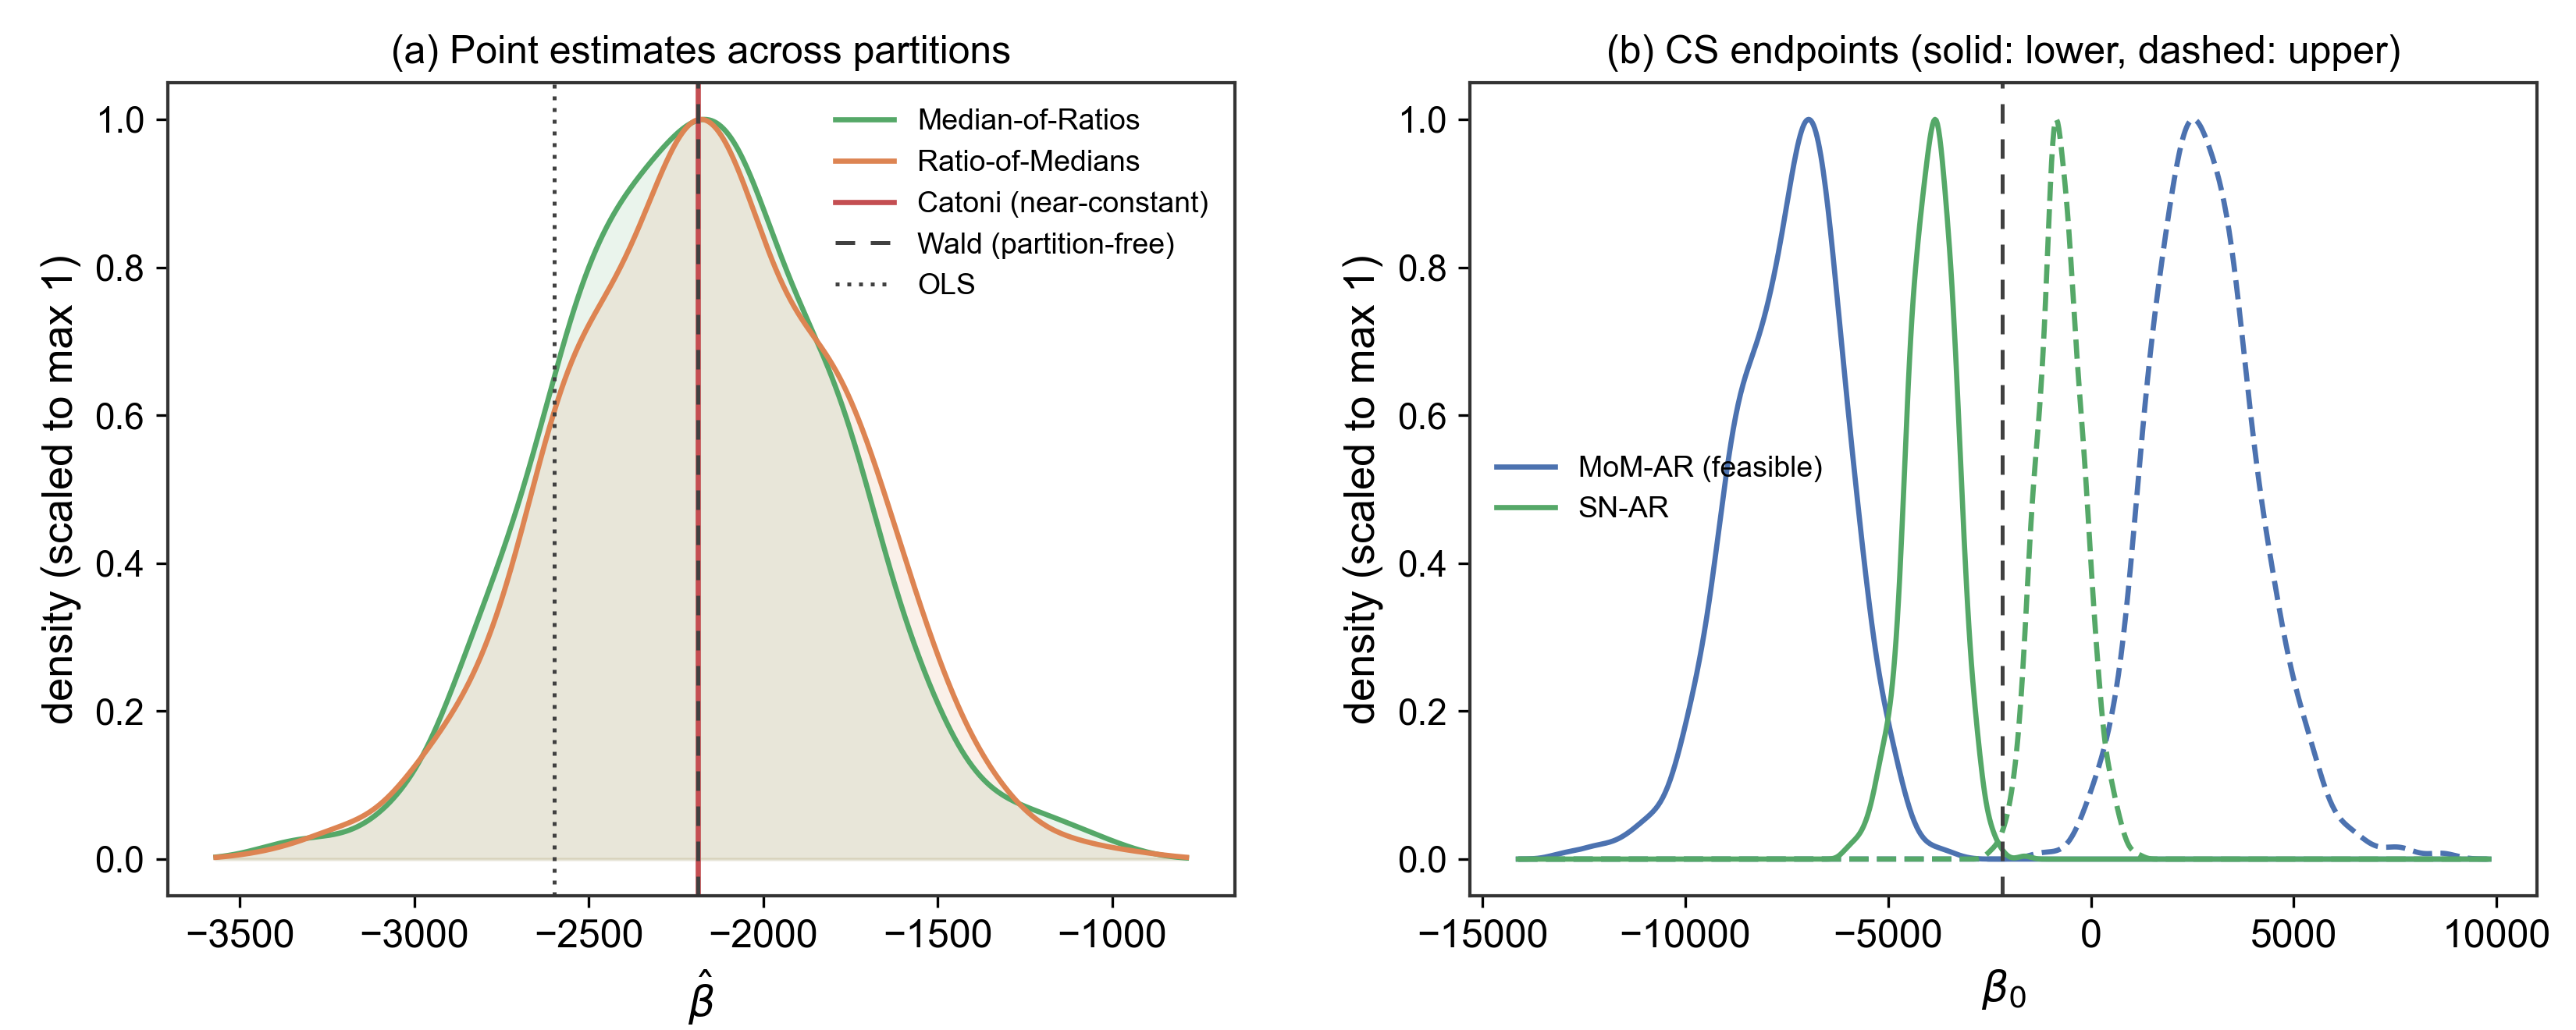
\includegraphics[width=\textwidth]{images/graphs/ae98_seed_sensitivity_incomem.png}
  \caption{Partition sensitivity for Labour income, \citet{angrist1998children} 1980 all-women sample, $B = 1{,}000$ random partitions. Panels as in Figure~\ref{fig:ak91_sensitivity}.}
  \label{fig:ae98_sensitivity_incomem}
\end{figure}

\subsubsection{Aggregated estimates and confidence sets}
\label{sss:ae98_aggregated}

Table~\ref{tab:ae98_aggregated} applies the same aggregation to the $B = 1{,}000$ partitions, for each of the five outcomes, against the single-partition Table~\ref{tab:ae98_robust}.

\todo[inline]{Expand: Here every aggregate lands on the partition-free Wald value: over the five outcomes the largest gap is $0.4\%$, Weeks worked at $-6.3872$ against $-6.3596$. That settles the reading offered for Table~\ref{tab:ae98_robust}, where on one partition Median-of-Ratios sat $21\%$ below the Wald estimate for Labour income and Ratio-of-Medians $31\%$ above it, and Ratio-of-Medians even reversed sign for ln(Family income) at $+0.0481$. Aggregated, those become $-2192.4$ and $-2171.4$ against $-2188.3$, and $-0.0248$ against $-0.0262$: the gaps were the draw of the partition, not the estimator, and aggregation removes them. The verdicts do not move, the self-normalised set excluding zero for the four labour-supply outcomes and containing it for ln(Family income), which is what Section~\ref{sss:ae98_sensitivity} anticipated in finding every partition already unanimous; what is new is that the reported numbers no longer depend on a seed. As in Section~\ref{sss:ak91_aggregated} the aggregated sets have close to the median per-partition length for every outcome and every test, and the feasible MoM-AR set still contains zero throughout.}

% Auto-generated by Code/replication_ae98_sensitivity.py -- do not edit by hand.

\begin{table}[htbp]
\centering
\caption{Aggregated estimates and aggregated 95\% confidence sets on the AE98 1980 all-women sample, over all $B = 1{,}000$ random partitions of Table~\ref{tab:ae98_sensitivity}, shared across outcomes (Definition~\ref{def:randomised} and Corollary~\ref{cor:agg_cs}, $\delta = 0.05$). Table~\ref{tab:ae98_robust} is the same quantities on a single partition. The Wald estimator and the standard AR test do not depend on the partition and are shown for reference; by Corollary~\ref{cor:agg_cs} the aggregated sets are guaranteed at $2\delta$, not $\delta$.}
\label{tab:ae98_aggregated}
\begin{tabular}{lccc}
\toprule
Outcome & Wald / Mean IV & Median-of-Ratios & Ratio-of-Medians \\
\midrule
Worked for pay & -0.1318 & -0.1335 & -0.1321 \\
Weeks worked & -6.3596 & -6.3872 & -6.4020 \\
Hours/week & -5.1872 & -5.1843 & -5.2561 \\
Labor income & -2188.3 & -2192.4 & -2171.4 \\
ln(Family income) & -0.0262 & -0.0259 & -0.0248 \\
\midrule
Outcome & MoM-AR (feasible) & SN-AR & AR (standard) \\
\midrule
Worked for pay & $[-0.374,\, 0.095]$ & $[-0.213,\, -0.067]$ & $[-0.184,\, -0.080]$ \\
Weeks worked & $[-17.18,\, 3.79]$ & $[-9.89,\, -3.48]$ & $[-8.68,\, -4.04]$ \\
Hours/week & $[-14.28,\, 3.59]$ & $[-8.22,\, -2.69]$ & $[-7.16,\, -3.22]$ \\
Labor income & $[-7319,\, 2722]$ & $[-3899,\, -772]$ & $[-3313,\, -1061]$ \\
ln(Family income) & $[-0.661,\, 0.583]$ & $[-0.234,\, 0.152]$ & $[-0.161,\, 0.109]$ \\
\bottomrule
\end{tabular}
\end{table}

